\subsection{Matthias Harvey}
	\textbf{Profile:}\\
	I have a passion for mathematics, science and software development. My special interests are computer graphics, simulations and artificial intelligence. I thrive on challenging projects. In my spare time I study French and Japanese, love music and play the guitar.
	\subsubsection{Contact}
	\begin{itemize}
		\item \href{mailto:matthiasharvey@gmail.com}{\textbf{Email} matthiasharvey@gmail.com}
		\item \href{https://github.com/MatthiasHarvey}{\textbf{Github} MatthiasHarvey}	
		\item \href{https://za.linkedin.com/in/matthias-harvey-68b30995}{\textbf{LinkedIn} Matthias Harvey}
	\end{itemize}
	\subsubsection{Photo}
	\begin{figure}[H]
		\centering
		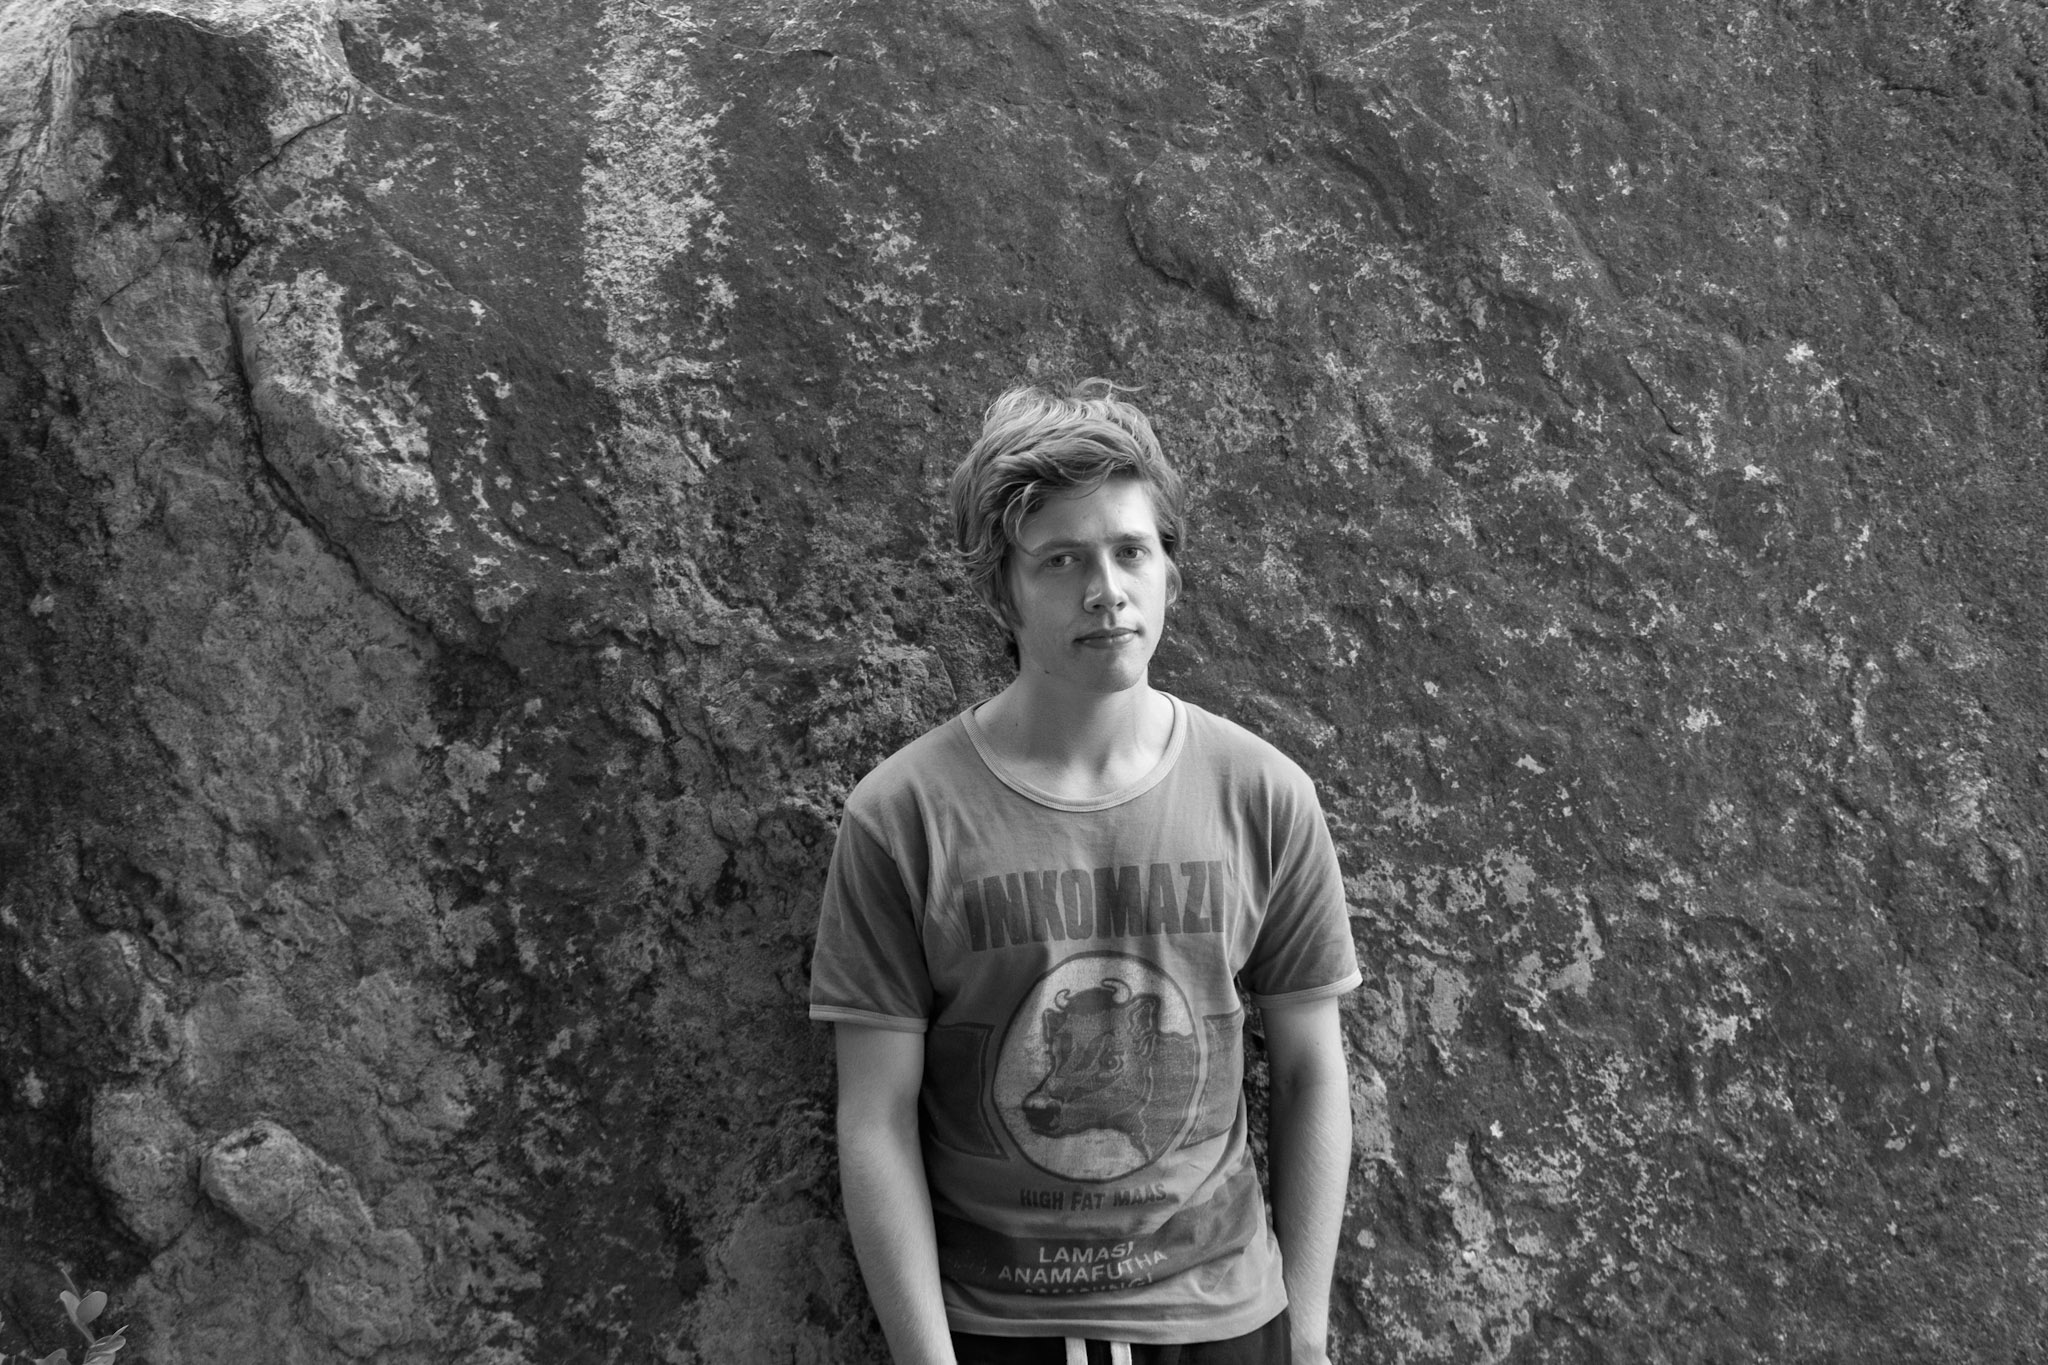
\includegraphics[width=0.7\textwidth]{../matthias.jpg}
		\caption{Matthias Harvey}
	\end{figure}
	\subsubsection{Interests}
	\begin{itemize}
		\item Computer graphics, artificial intelligence, game programming, simulations
		\item Mathematics
		\item Physics
		\item French - read, write. Speak - intermediate. Japanese – beginner
	\end{itemize}
	\subsubsection{Technical Skills}
	
	\begin{tabular}{| l | l | l |}
		Java   & C\#     & F\#                          \\
		Git    & C++, NASM     & Haskell                     \\
		OpenGL & SQL     & HTML, CSS, JavaScript, PHP   \\
		Django & Unity3D & Python                     
	\end{tabular}

	\subsubsection{Past Experience \& Achievements}
	\begin{itemize}
		\item \textbf{Past Experience}
		\begin{itemize}
			\item Research Assistant for the SSFM Research Group
			\begin{itemize}
				\item University of Pretoria
				\item Assisting Prof. S. Gruner and Dr. N. Timm with research pertaining to Formal Methods - specifically 3-Valued Bounded Model Checking
			\end{itemize}
			\item Web Developer for Ms. Vreda Pieterse (Software engineering lecturer)
			\begin{itemize}
				\item University of Pretoria
				\item July 2014 - Present
			\end{itemize}
			\item Teaching Assistant
			\begin{itemize}
				\item University of Pretoria
				\item February 2015 - Present
			\end{itemize}
			
			\item Developer at Monkey \& River during 2015
			\begin{itemize}
				\item Pretoria
				\item Helped develop a web-based system (using ASP.NET MVC) to compare municipalities and districts in SA. See demo here: \href{http://salgabarometerdemo.org.za/RatingTool}{RatingTool}
				\item June 2015 - December 2015
			\end{itemize}
			
			\item Intern at Agnomen Design
			\begin{itemize}
				\item Agnomen Design. An indie-game studio based in Cape Town
				\item $ \pm 3 $ months experience during holidays since 2014
			\end{itemize}
		\end{itemize}
		
		\item \textbf{Achievements}
		\begin{itemize}
			\item High school science expo – silver at nationals (Electricity from cardboard)
			\item Completed an online course: Creative Coding (from Monash University) 2014
			\item Placed 5th at the national finals of the Standard Bank IT Challenge 2015
			\item Currently team leader of six selected students developing a web-based peer review system for the University of Pretoria
			\item Invited to Golden Key
			\item Distinction average throughout university
		\end{itemize}
	\end{itemize}
	
	\subsubsection{Non-technical Skills/Hobbies}
	\begin{itemize}
		\item Rock Climbing, parkour, mountain biking
		\item Guitar, music production
		\item Computer generated art through coding
	\end{itemize}